%===================================== CHAP 2 =================================

\chapter{Literature Review/Background}

%Web and experience, enric pliaza, ralph bergmann, CBR stuff cooking recepies

%Mining stories from web
\section{Related work}
Discuss other articles that touch on the same subject

\subsection{Wikimedia}


\subsection{SMILA} \label{smila}

\begin{figure}[h]
\caption{An overall overview of the SMILA architecture}
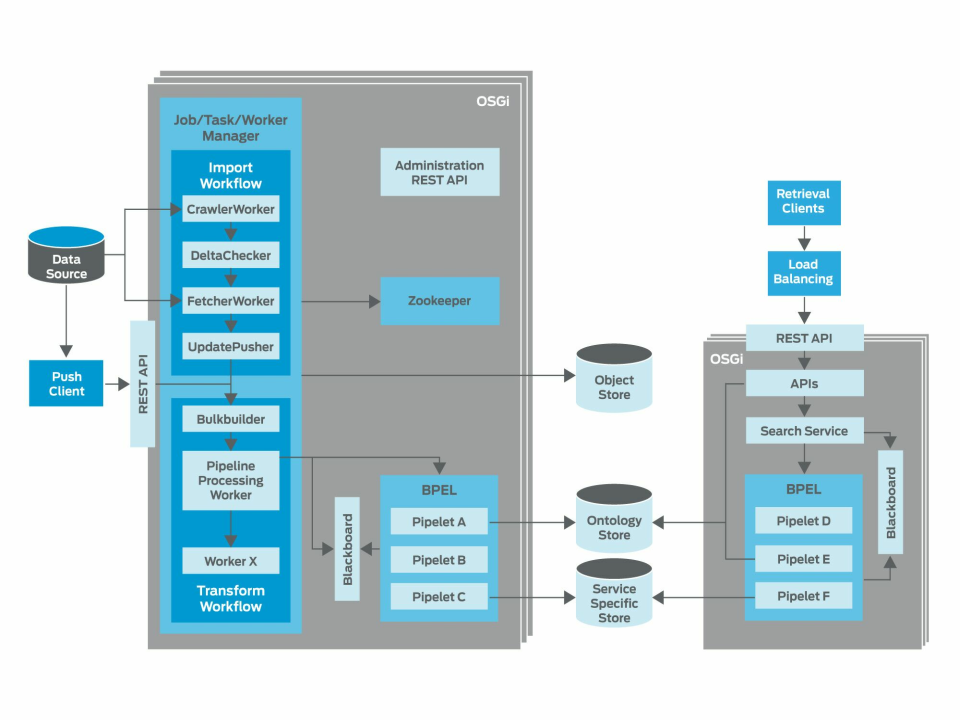
\includegraphics[width=\textwidth]{SMILA_Architecture}
\end{figure}

%%fix sånn abbrevation for SMILA

%%når jeg snakker om mine erfaringer med smila gjør jeg det i implementation.

%%Skriv om dette til å passe til sin nye kontekst
In the early stages of the project, an existing project called SMILA was explored. SMILA crawls the web to extract information and then stores the information in an index. It has a REST API to control the system and for searching the index. The SMILA architecture is also based on the pipeline architecture containing the following processes jobs, crawling, storage, indexing and querying. With SMILA being very complex, it gains asynchronicity as its biggest benefit from the pipeline architecture. The SMILA pipeline also allows custom made pipelets to be inserted into the pipeline. A pipelet is a sub process inside a pipeline. By creating pipelets, the behaviour of SMILA could be tailored into extracting the relevant information from Wikipedia.

By only writing pipelets and then make SMILA use them when crawling Wikipedia, the project could concentrate the effort on identifying and indexing the examples. Unfortunately SMILA is an old and complex system, and is rarely updated anymore. When problems running SMILA appeared, it was quite troublesome to understand why and fix the issue. This ironically lead to all the effort in the starting phase being used on making SMILA run properly, instead of looking into the characteristics of examples. 

\section{Tools}

\subsection{ElasticSearch} \label{elasticsearch}
%%JSON abbrevation
ElasticSearch is a tool used in this project for indexing the examples. ElasticSearch is built on top of Apache Lucene(https://lucene.apache.org), which is a information retrieval library, written in Java. Internally in ElasticSearch, data is stored as structured JSON\footnote{JSON - JavaScript Object Notation} documents. The API for communicating with ElasticSearch is a RESTful\footnote{REST - representational state transfer} API using JSON over HTTP. The API can be used for configuring ElasticSearch, building the index and querying it. 
%%Ta med i erfaring seksjon om dette at siden alt dette bruker json og webserveren bruker javascript via node, er alt veldig enkelt og konsistent.

ElasticSearch is built for scalability. This means that it can handle the dataset and interactions growing. This is because it acts as a cluster of many nodes. If the system needs to scale, new nodes can easily be added, and ElasticSearch will distribute resources to the newly added ndoes. However this projects does not need or take advantage of this scaling, and will only be using one node.

When searching in ElasticSearch, there is mainly two ways of doing this. The first one is by using \textit{filter}. The \textit{filter} is utilizing \textit{term} to decide whether a document should be returned or not. Searching with \textit{term} is very similar to how one would use SQL. %Trenger denne forklaring?
Searches can for instance consist of text strings, numbers, ranges or dates, and ElasticSearch will return everything that matches. It also allows for boolean operators and nesting of these. Using a \textit{filter} is very quick and should be used if the relevance of the documents is not important. If relevance score is important then the second option, \textit{query}, should be chosen. If a \textit{query} is combined with a \textit{term}, ElasticSearch is looking for the exact value in its index. A score is then returned based on the documents TF/IDF relevance to the term. See section \label{tfidf} for an explanation of this algorithm.%Burde det referes på denne måten?
If a \textit{match} is used instead, an analysis will be performed, creating a list of terms from the query, and then executing low-level queries for each of the terms. The results are combined to produce the final relevance score. These two methods can also be combined or extended with other methods to customize the search further.


\subsection{NPM and Node.js}

\section{Techniques}

\subsection{Pipeline} \label{pipeline}
Describe a software pipeline. Advantages and stuff.\\
How should i use references for this?

\subsection{TF/IDF} \label{tf/idf}
TF/IDF is an algorithm which calculates how important an word is to a document based on the document itself and the collection it is part of. Based on this it is possible to decide how likely it is for the document to be relevant. TF/IDF is used as the standard similarity algorithm in ElasticSearch, \ref{elasticsearch}.

TF/IDF is can be divided into two parts, \textit{term frequency} and \textit{inverse document frequency}. \textit{Term frequency} is how often a term appears in a document. The more instances the document has of the word, the higher is the chance of the document being relevant. \texit{Inverse document frequency} looks at how often a term appears in the whole collection of documents. The more often a term appears, the less relevant is the term. This means the common terms will have less weight than rare ones, when calculating the likelihood of the documents relevance. 

\cleardoublepage